% !TEX encoding = UTF-8
% !TEX TS-program = pdflatex
% !TEX root = ../../tesi.tex

\section{Propensione all'innovazione}
Sync Lab è un'azienda in costante aggiornamento che guarda all'innovazione con grande interesse, per garantire soluzioni software sempre rivoluzionarie. Simbolo di questo sforzo da parte dell'azienda è anche la grande quantità di collaborazioni con le principali università d'Italia (università degli studi di Padova, politecnico di Milano, università degli studi Federico II, ecc.) e vari enti europei. \\

\begin{figure}[!h]
  \centering
  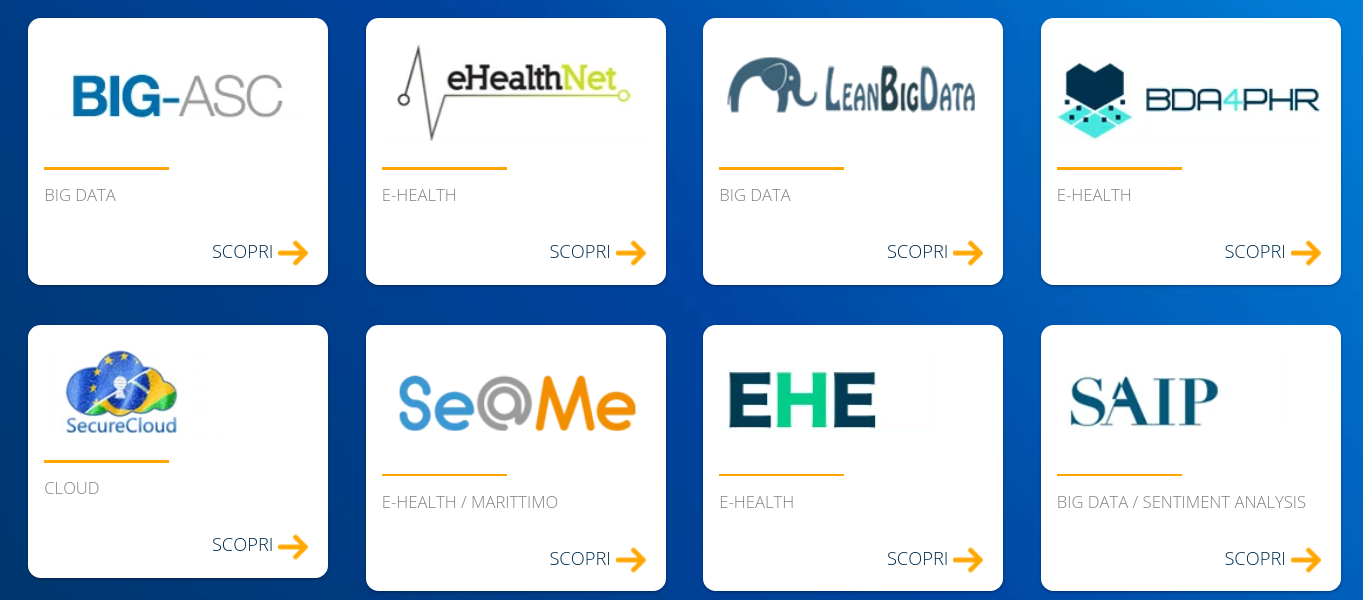
\includegraphics[width=\textwidth]{capitolo1/prodotti-ricerca-sviluppo.png}
  \caption{Alcuni progetti di ricerca e sviluppo di Sync Lab}
  \textbf{Fonte}: \href{https://www.synclab.it/ricerca-e-sviluppo.php}{https://www.synclab.it/ricerca-e-sviluppo.php}
\end{figure}

Per adempiere al meglio al difficile compito di restare sempre aggiornati sulle ultime tecnologie, Sync Lab è divisa in tre dipartimenti:
\begin{itemize}
  \item \textbf{\textit{Research and Development (R\&D)}}: dove l'azienda promuove nuovi prodotti eseguendo ricerca e sviluppo in più settori, alimentando così il profilo aziendale e le proprie competenze nel mercato;
  \item \textbf{\textit{Lab}}: in cui l'azienda mette in atto i risultati derivanti dal dipartimento \textit{R\&D}, promuovendo soluzioni che migliorino ed estendano l'innovazione tecnologica;
  \item \textbf{\textit{Start-up}}: dove l'azienda collabora e promuove le \textit{start-up} con maggiore successo in termini di innovazione, sia in Italia che all'estero.
\end{itemize}  

L'azienda, inoltre, sta approfondendo sempre di più gli ambiti di \textit{Cybersecurity}, \textit{E-Health}, \textit{Blockchain} e \textit{Big Data}, formando degli appositi progetti di ricerca nelle diverse sedi per sperimentare e imparare nuove tecnologie. \\

Un evento che ho trovato interessante e mi è piaciuto molto durante il mio tirocinio, è stato il "Paola presenta". 
Questa ricorrenza, che in genere è settimanale, consiste in un'ora di presentazione su un argomento proposto da un dipendente. L'argomento della presentazione può riguardare qualcosa sulla quale sta lavorando, oppure semplicemente si è interessato. 
Ogni dipendente è libero di partecipare e, su richiesta, può presentare lui stesso un argomento a piacere. Questo evento l'ho trovato molto interessante e dimostra quanto i colleghi di Sync Lab vogliano sempre stare aggiornati ed informati su tutto quello che interessa il mondo informatico. 
Personalmente ho partecipato a tre di queste presentazioni: una dove hanno introdotto la tecnologia \textit{Blockchain}, tenuta dal mio \textit{tutor} aziendale Fabio Pallaro, un'altra dove hanno spiegato come funzionano gli strumenti che compongono la \textit{Elastick Stack} e l'ultima dove hanno parlato dell'analisi statica del codice con la piattaforma \textit{SonarQube}. \\

Questa propensione all'innovazione l'ho avvertita anche nel mio progetto di stage, dove non ho trattato tecnologie usuali, ma ho dovuto studiare e approfondire tecnologie che attualmente non sono così diffuse in ambito \textit{enterprise}, ma sicuramente rappresentano un'importante \textit{milestone} nella storia dell'informatica.